\section{Visualisierung der Mengen}
\label{sec:visualisierung}
In den vorherigen Abschnitten wurden Bilder von der Mandelbrot-Menge sowie der Julia- und Fatou-Mengen gezeigt.
Nachfolgend wird beschrieben wie diese Mengen visualisiert werden.
Bei diesen Visualisierungen handelt es sich um \emph{Fraktale}, was bedeutet dass, unabhängig vom Vergrösserungsfaktor, stets neue Details und Strukturen erscheinen.
Diese Strukturen sind häufig selbstähnlich, heisst sie sind eingebettet in grössere Strukturen, die ähnlich aussehen.

\subsection{Visualisierung der Julia- und Fatou-Mengen}

\begin{aufgabe}
    Visualisierung Julia- und Fatou-Mengen
    \begin{enumerate}
        \item Funktion $f(z)$ wählen
        \item Die reelle und imaginäre Achse der $z$-Ebene plotten
        \item $f^n(z_i)$ für jeden Punkt $z_i$ dieses Koordinatensystems berechnen
        \item Punkte $z_i$ einfärben, je nachdem wie schnell und ob sie divergieren
    \end{enumerate}
\end{aufgabe}
Zu beachten ist, dass $n$ in der Theorie gegen unendlich geht, in der Praxis ist dies natürlich nicht möglich, je nach Rechenleistung muss ein genügend grosser Wert für $n$ gewählt werden.

Je nach gewählter Funktion und Farbschema können so sehr eindrückliche Bilder erstellt werden, wie zum Beispiel in Abbildung \ref{fig:bsp_julia}.
Interessant wird es besonders dann, wenn die Julia-Menge \emph{nicht zusammenhängend} ist (siehe Abschnitt \ref{sec:julia_connected}).
In diesem Fall besteht die Julia-Menge häufig nur aus einzelnen Punkten, während die übrigen Punkte zur Fatou-Menge gehören.

\begin{figure}
    \centering
    
\includegraphics[width=0.95\textwidth]{papers/julia/imgs/julia3.jpg}

    \caption{Beispiel einer Julia-Menge}
    \label{fig:bsp_julia}
\end{figure}

\subsection{Visualisierung der Mandelbrot-Menge}
\label{sec:visualisierung_mandel}

\begin{aufgabe}
    Visualisierung Mandelbrot-Menge
    \begin{enumerate}
        \item Beginne mit $f_c(z) = z^2 + c$
        \item Die reelle und imaginäre Achse der $c$-Ebene plotten
        \item $f^n_{c_i}(0)$ für jeden Punkt $c_i$ dieses Koordinatensystems berechnen
        \item Punkte $c_i$ einfärben, je nachdem wie schnell und ob sie divergieren
    \end{enumerate}
\end{aufgabe}
Der Ablauf ist im wesentlichen gleich wie bei den Julia- und Fatou-Mengen, der grosse Unterschied liegt darin, dass hier der Parameterraum bzw. die $c$-Ebene abgebildet wird.
Auch hier gilt in der Theorie $n \to \infty$, es muss wieder ein genügend grosser Wert für $n$ gewählt werden.

Je nach Farbschema führt auch dies zu sehr eindrücklichen Bildern, wie zum Beispiel Abbildung \ref{fig:bsp_mandelbrot}.

\begin{figure}
    \centering
    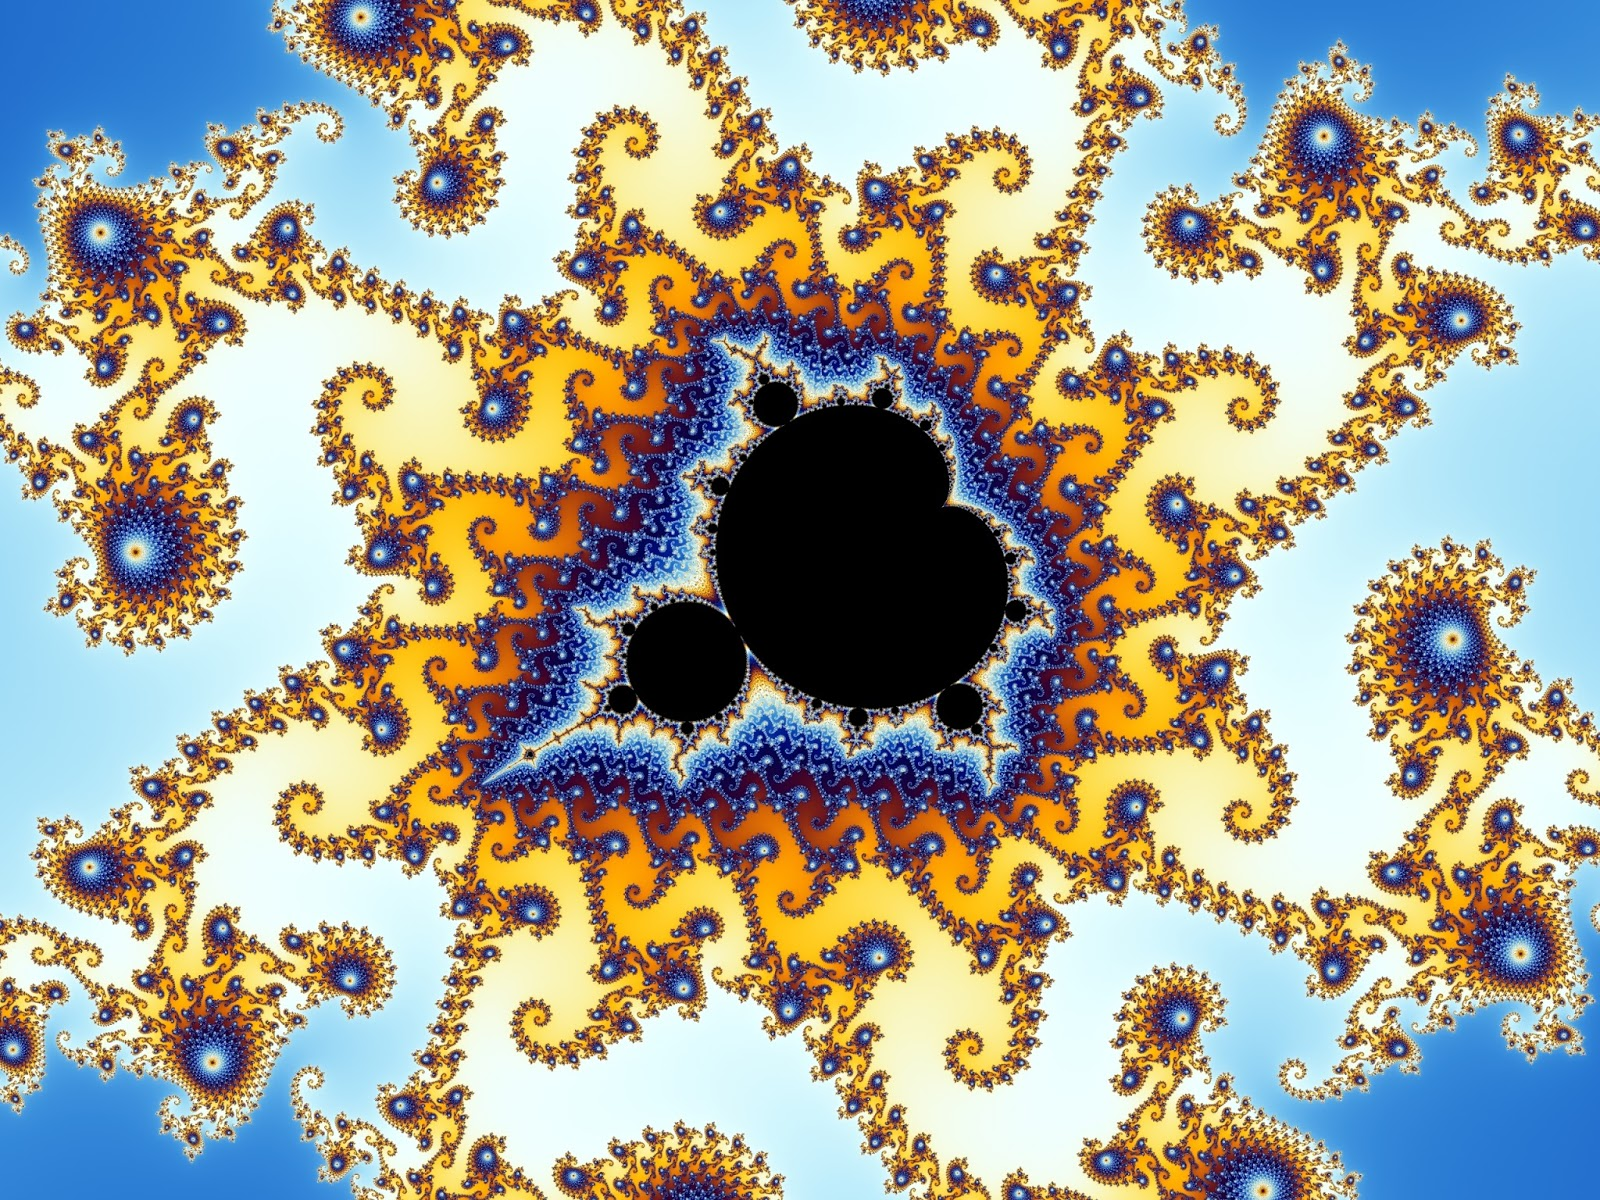
\includegraphics[width=0.95\textwidth]{papers/julia/imgs/mandelbrot1.jpg}

    \caption{Beispiel der Mandelbrot-Menge}
    \label{fig:bsp_mandelbrot}
\end{figure}
